\section{Технологическая часть}
В данной части рассматривается выбор средств реализации, описывается структура классов программы и приводится интерфейс программного обеспечения.

\subsection{Средства реализации}

Для написания данного курсового проекта был выбран язык C++~\cite{cpp-lang}.
Выбор данного языка программирования обусловлен следующим образом:
\begin{itemize}
	\item поддерживает объектно-ориентированную модель разработки, что позволяет структурировать программу и дает возможность эффективного написания качественного программного обеспечения;
	\item позволяет эффективно использовать ресурсы системы благодаря широкому набору функций и классов из стандартной библиотеки;
	\item обладает высокими показателями вычислительной производительности, а так как требуется быстродействие задач генерации реалистичных изображений, то язык C++ необходим.
\end{itemize}

В качестве среды разработки был использован Qt Creator~\cite{qt-creator}. 
Он обладает всем необходимым функционалом для написания, профилирования и отладки программ, а также создания графического пользовательского интерфейса.
Данная среда поставляется с фреймворком Qt~\cite{qt-framefork}, который содержит в себе все необходимые средства, позволяющие работать непосредственно с пикселями изображения.
Для упрощения сборки проекта программного обеспечения использовалась утилита qmake~\cite{qmake}.

\subsection{Структура программы}

На рисунке~\ref{fig:struct} представлена схема разработанных классов.

\begin{figure}[h]
	\centering
	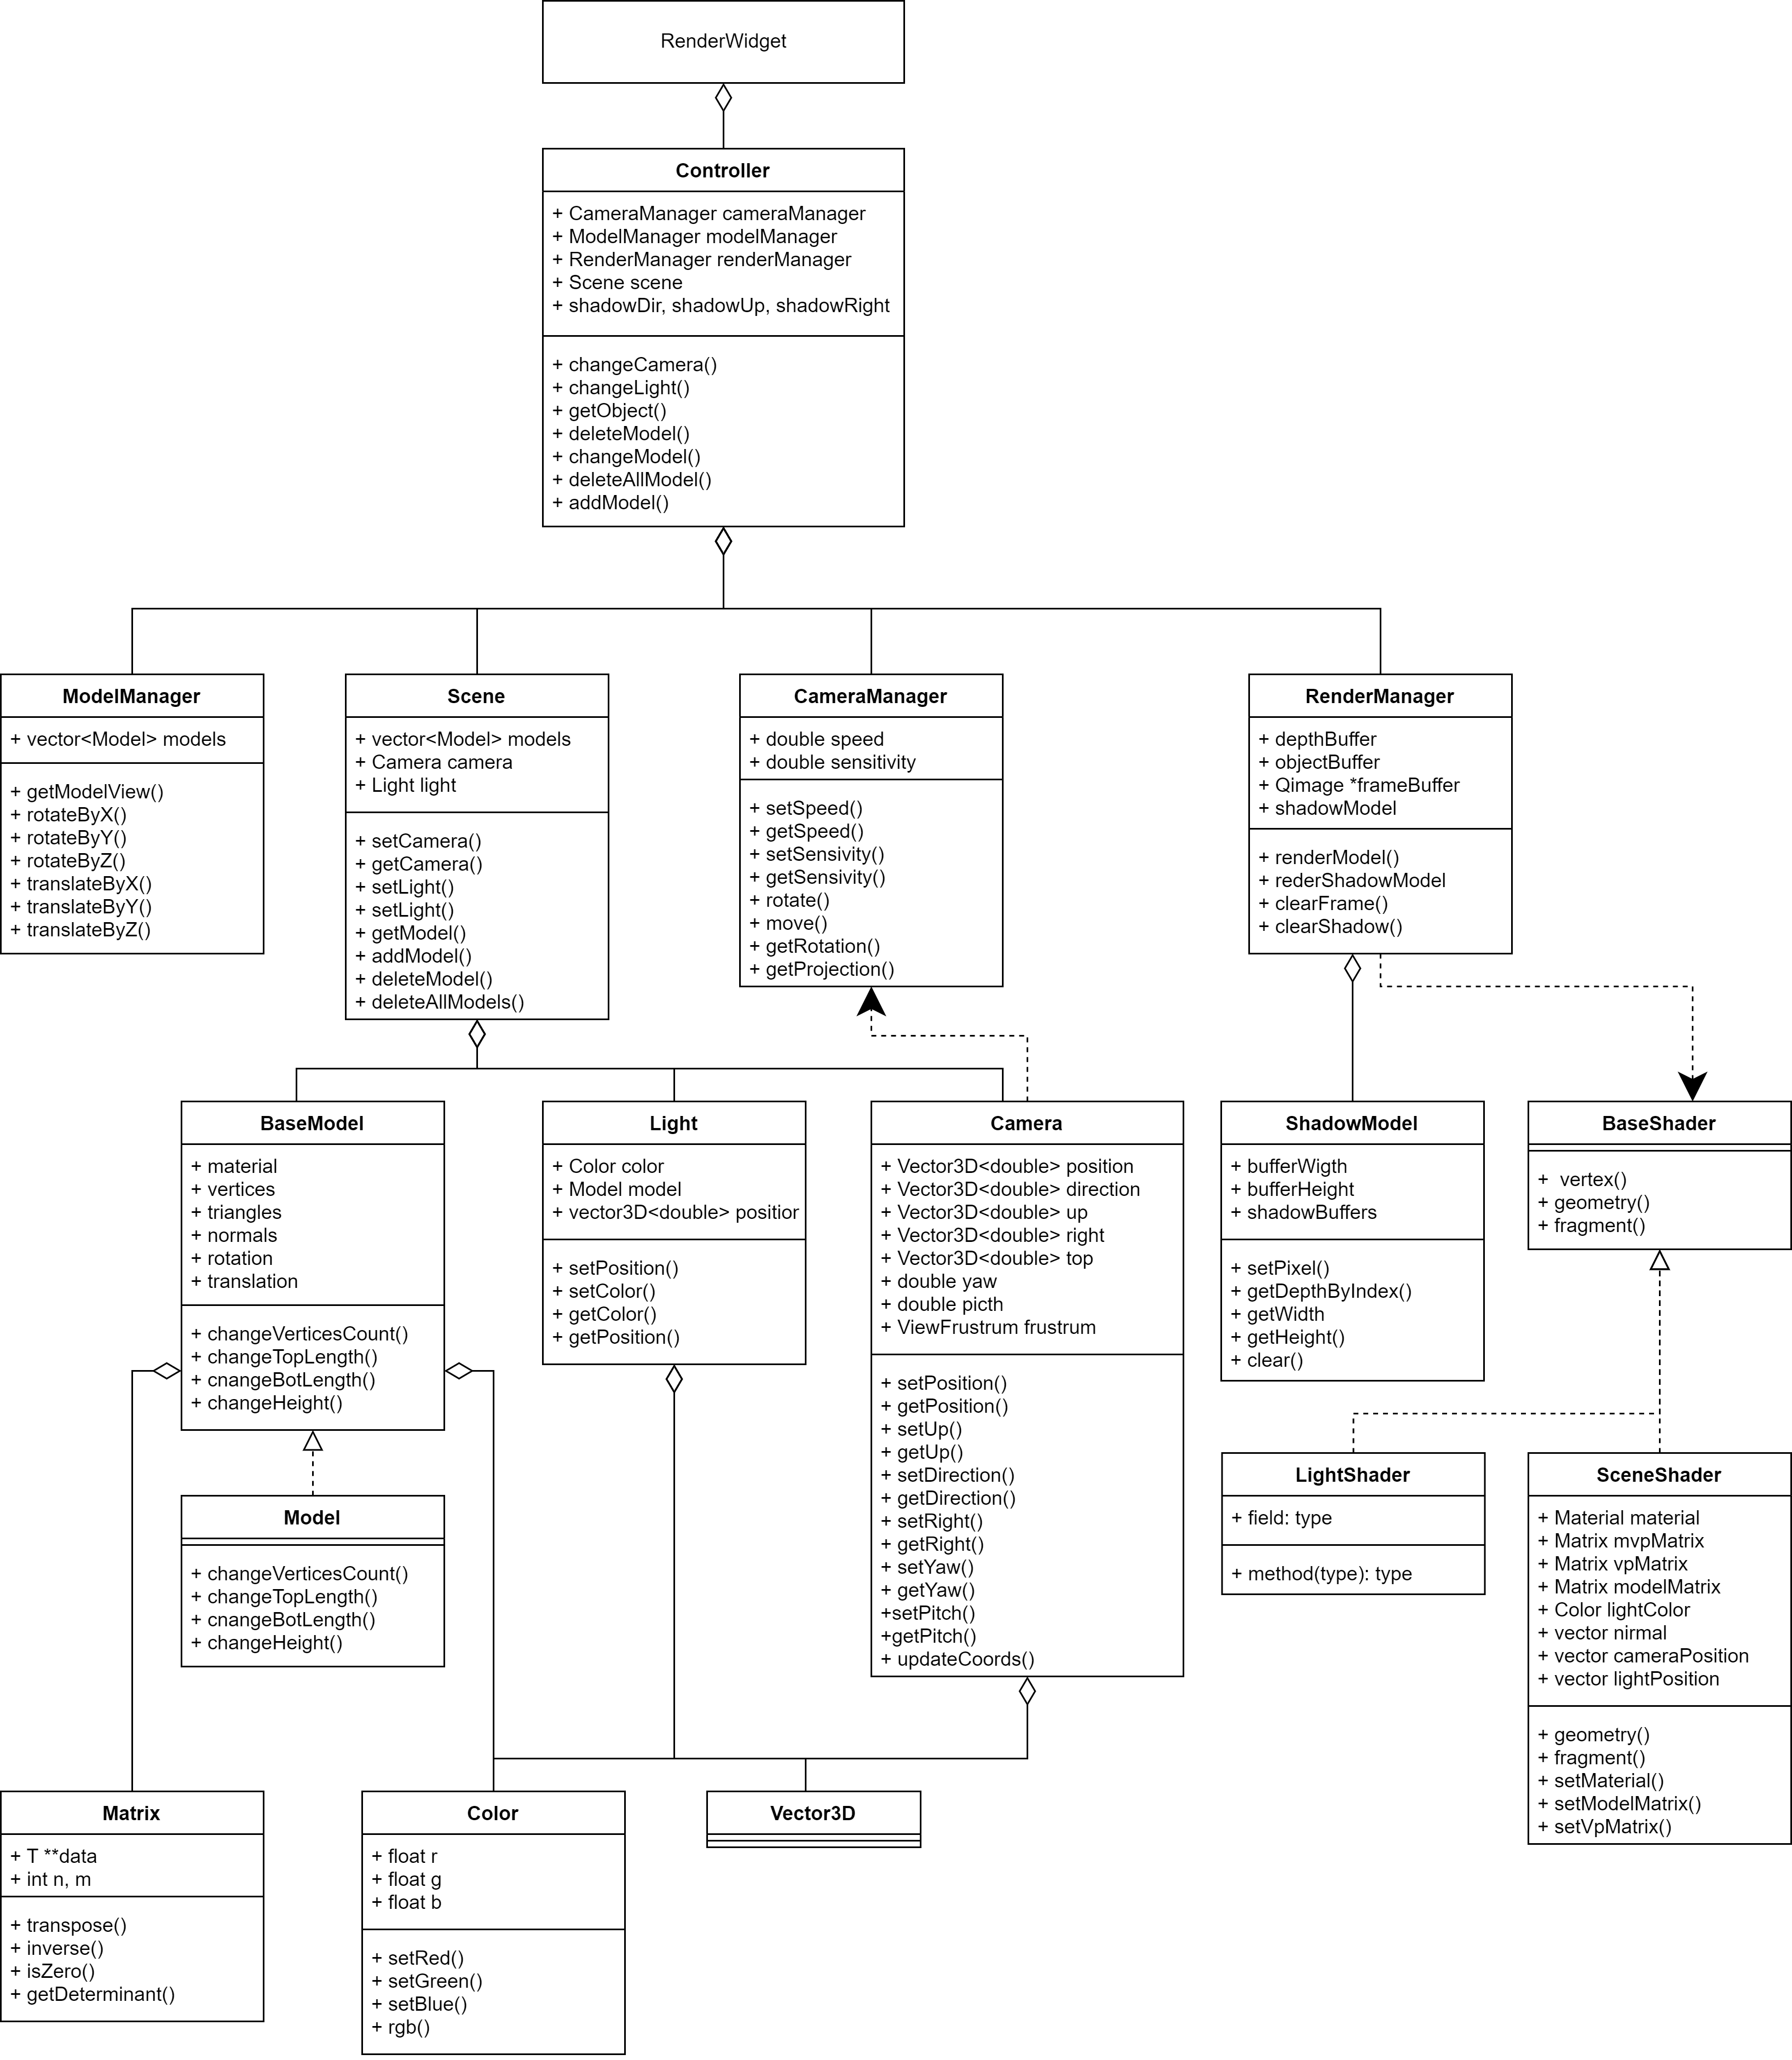
\includegraphics[width=0.9\textwidth]{img/algorithms/struct.png}
	\caption{Схема классов программы}
	\label{fig:struct}
\end{figure}

Разработанная программа состоит из следующих классов.
\begin{itemize}
	\item Базовые математические классы:
	\begin{itemize}
		\item Matrix --- класс матриц;
		\item Vector3D --- класс векторов трехмерного пространства;
		\item Vector4D --- класс векторов в однородных координатах.
	\end{itemize}
	\item Классы для работы с моделями
	\begin{itemize}
		\item BaseModel --- базовый класс моделей с возможностью перемещения по сцене и изменения спектральных характеристик;
		\item Model --- класс модели с параметрами радиус верхнего и нижнего оснований, высота и число боковых граней, которые можно меняться.
	\end{itemize}
	\item Вспомогательные классы сцены
	\begin{itemize}
		\item Camera --- класс камеры с возможностью перемещения по сцене;
		\item Light --- класс источника освещения с возможностью перемещения по сцене и изменения цвета.
	\end{itemize}
	\item Классы рейдеров
	\begin{itemize}
		\item BaseShader --- базовый класс шейдера для преобразования вершин и вычисления интенсивности пикселей;
		\item SceneShader --- класс шейдера для визуализации сцены;
		\item LightShader --- класс шейдера для визуализации источника освещения.
	\end{itemize}
	\item Классы управления сценой
	\begin{itemize}
		\item ModelManager --- класс для осуществления аффинных преобразований;
		\item CameraManager --- класс для осуществления видовых и перспективных преобразований;
		\item RenderManager --- класс для визуализации сцены;
		\item Scene – класс управления объектами сцены.
	\end{itemize}
	\item Классы интерфейса
	\begin{itemize}
		\item Controller --- класс для взаимодействия управляющих классов с классами интерфейса;
		\item RenderWidget --- класс виджета сцены для вывода буфера кадра;
		\item MainWindow --- класс главного окна сцены.
	\end{itemize}
\end{itemize}

\subsection{Реализация алгоритмов}

На листингах \ref{lst:render-scene} -- \ref{lst:z-buffer} приведена реализация алгоритма визуализации сцены по схеме алгоритма синтеза изображения, который показан на рисунке~\ref{fig:alg_scene}.
В листинге \ref{lst:z-buffer} приведена многопоточная реализация алгоритм с Z-буфером.

Основной поток создает вспомогательные потоки и разбивает растеризацию полигона между ними, данную реализацию можно рассмотреть на листингах~\ref{lst:render-triangle_1}--\ref{lst:render-triangle_2}.
В качестве аргументов потоку передается:
\begin{itemize}
	\item startCol --- номер строки буфера для начало работы;
	\item endCol --- номер строки буфера для конца работы потока;
	\item startRow --- номер столбца буфера для начало работы потока в строках $[startCol;endCol)$;
	\item endRow --- номер столбца буфера для конца работы потока в строках $[startCol;endCol)$;
\end{itemize}
По аргументам будет определен объем работы, выполняемый конкретным вспомогательным потоком.

На листингах \ref{lst:render-shadow} -- \ref{lst:render-shadow-triangle-2} представлена реализация алгоритма визуализации теней на сцене с использованием карты теней.

На листингах \ref{lst:model-move} -- \ref{lst:model-rotate-1} представлены реализация поворота и перемещения модели. На листингах \ref{lst:camera-move} -- \ref{lst:camera-proj} представлены реализации движения и поворота камеры, вычисления перспективной проекции пространства камеры.

\clearpage

\lstinputlisting[label=lst:render-scene,caption=Реализация визуализации сцены, firstline=253,lastline=284]{../controller/controller.cpp}

\clearpage

\lstinputlisting[label=lst:render-model,caption=Реализация визуализации модели на сцене, firstline=21,lastline=40]{../scene/render/rendermanager.cpp}

\clearpage

\lstinputlisting[label=lst:render-triangle_1,caption=Реализация визуализации полигона модели на сцене (Часть 1), firstline=111,lastline=135]{../scene/render/rendermanager.cpp}

\lstinputlisting[label=lst:render-triangle_2,caption=Реализация визуализации полигона модели на сцене (Часть 2), firstline=136,lastline=148]{../scene/render/rendermanager.cpp}

\clearpage

\lstinputlisting[label=lst:z-buffer,caption=Реализация алгоритма с z-буфером, firstline=190,lastline=213]{../scene/render/rendermanager.cpp}

\clearpage

\lstinputlisting[label=lst:render-shadow,caption=Реализация визуализации теней на сцене, firstline=286,lastline=314]{../controller/controller.cpp}

\clearpage

\lstinputlisting[label=lst:render-shadow-model,caption=Реализация визуализации теней для модели на сцене, firstline=43,lastline=61]{../scene/render/rendermanager.cpp}

\clearpage

\lstinputlisting[label=lst:render-shadow-triangle-1,caption=Реализация визуализации теней для полигона модели на сцене с использованием карты теней (Часть 1), firstline=150,lastline=169]{../scene/render/rendermanager.cpp}

\lstinputlisting[label=lst:render-shadow-triangle-2,caption=Реализация визуализации теней для полигона модели на сцене с использованием карты теней (Часть 2), firstline=170,lastline=187]{../scene/render/rendermanager.cpp}

\clearpage

\lstinputlisting[label=lst:model-rotate-1,caption=Реализация афинного преобразования --- поворота модели (Часть 1), firstline=8,lastline=34]{../scene/model/modelmanager.cpp}

\lstinputlisting[label=lst:model-rotate-2,caption=Реализация афинного преобразования --- поворота модели (Часть 2), firstline=35,lastline=42]{../scene/model/modelmanager.cpp}

\begin{lstlisting}[label=lst:model-move,caption=Реализация афинного преобразования --- перемещение модели]
inline void translateByX(BaseModel &model, const double &translation) const {
	model.setTranslation(model.getTranslation() + Vector3D<double>(translation, 0, 0));
}
inline void translateByY(BaseModel &model, const double &translation) const {
	model.setTranslation(model.getTranslation() + Vector3D<double>(0, translation, 0));
}
inline void translateByZ(BaseModel &model, const double &translation) const {
	model.setTranslation(model.getTranslation() + Vector3D<double>(0, 0, translation));
}
\end{lstlisting}

\clearpage

\lstinputlisting[label=lst:camera-rotate,caption=Реализация поворота камеры, firstline=13,lastline=38]{../scene/camera/cameramanager.cpp}

\clearpage

\lstinputlisting[label=lst:camera-move,caption=Реализация движения камеры, firstline=40,lastline=54]{../scene/camera/cameramanager.cpp}

\lstinputlisting[label=lst:camera-proj,caption=Реализация алгоритма вычисления перспективной проектции, firstline=92,lastline=103]{../scene/camera/cameramanager.cpp}

\clearpage

\subsection{Интерфейс программного обеспечения}

При запуске программы на виджете сцены отображается источник освещения и система координат в левом нижнем углу. Источник освещения отображается как пирамида цвета источника.
Для операциям над объектами в левой части интерфейса определены разделы (создания и изменения объекта) и для управления камерой или освещением используются разделы в правой части экрана (рисунок~\ref{fig:example}).

\begin{figure}[h]
	\centering
	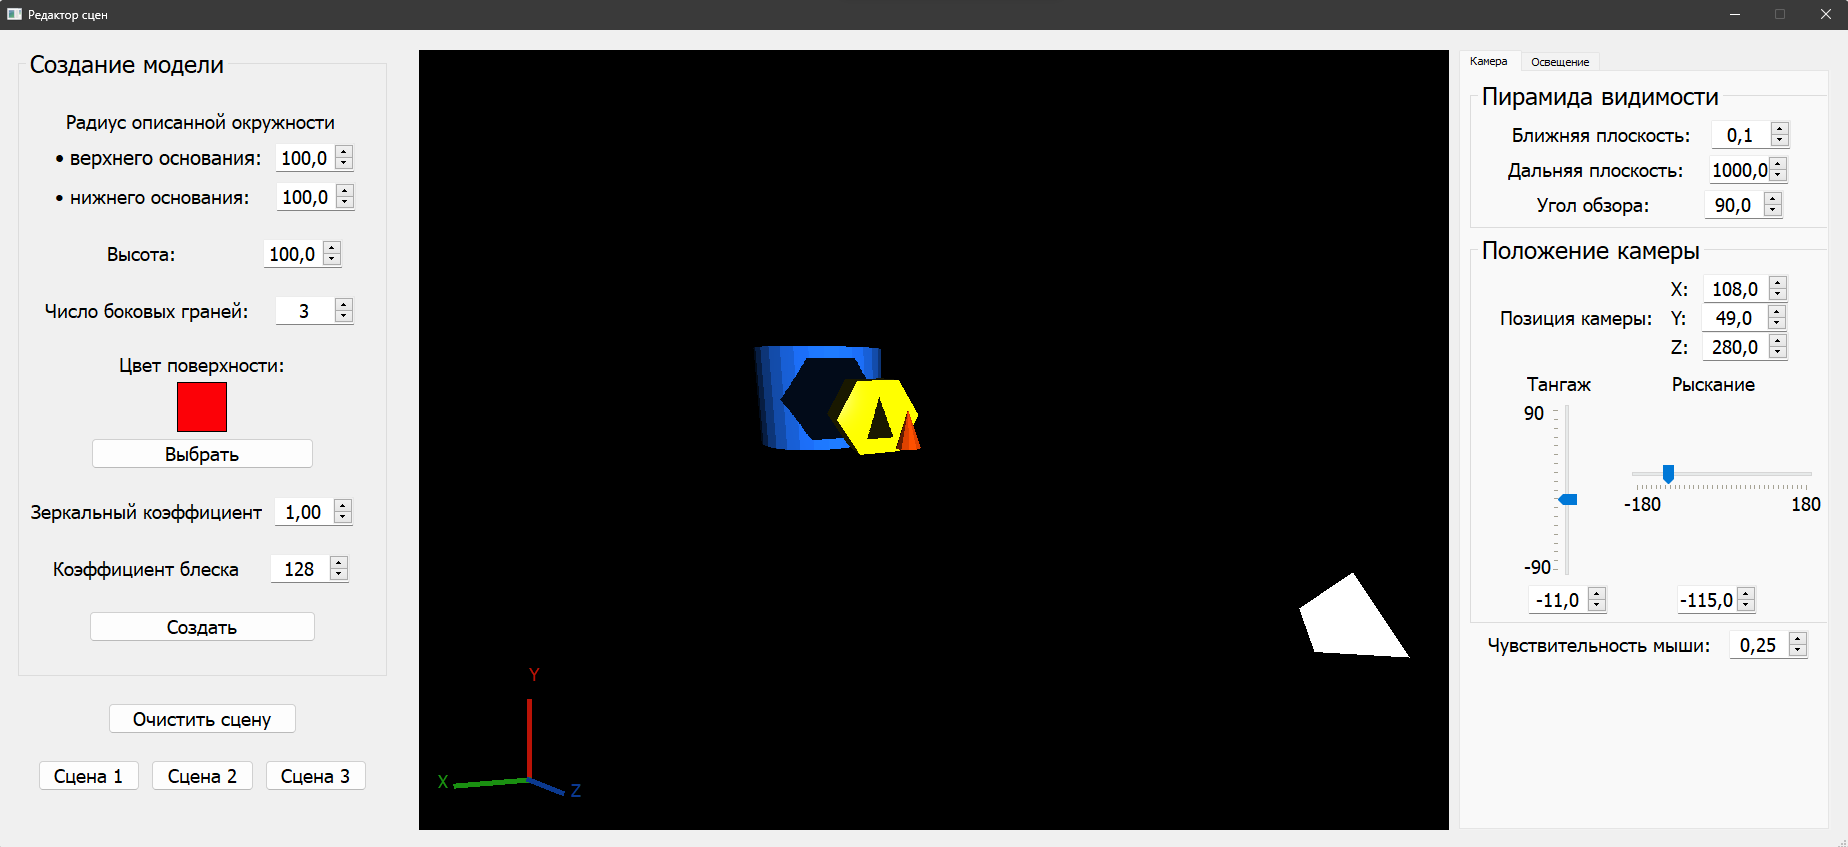
\includegraphics[width=0.95\textwidth]{img/examples/example.png}
	\caption{GUI}
	\label{fig:example}
\end{figure}

Для создания модели пользователю необходимо ввести в разделе <<Создание модели>> ее геометрические и спектральные характеристики: радиусы верхнего и нижнего оснований, высоту, число боковых сторон, цвет поверхности, коэффициент блеска и зеркальный коэффициент, раздел показан на рисунке~\ref{fig:create}.

\clearpage

\begin{figure}[h]
	\centering
	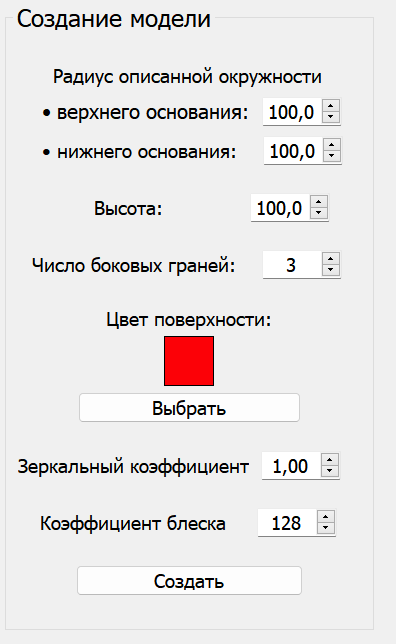
\includegraphics[width=0.3\textwidth]{img/examples/create.png}
	\caption{Раздел создание модели}
	\label{fig:create}
\end{figure}

При нажатии правой кнопкой мыши по модели на виджете сцены в разделе <<Создание модели>>s отобразится секция с редактированием модели, раздел показан на рисунке~\ref{fig:change-model}. 
Для возврата в секцию создания необходимо нажать правой кнопкой мыши по пустой части виджета сцены.

Для перемещения по сцене используются клавиши: W – вперед, S – назад, A – влево, D – вправо. Для поворота камеры необходимо зажать левую кнопку мыши и переместить мышь.

\clearpage
\begin{figure}[h]
	\centering
	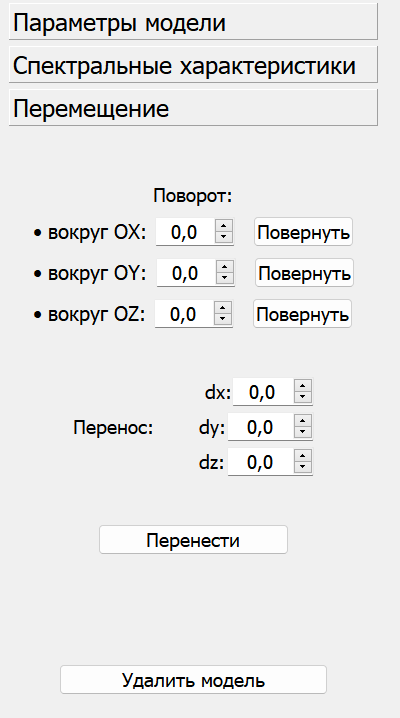
\includegraphics[width=0.3\textwidth]{img/examples/change-model.png}
	\caption{Раздел редактирование модели}
	\label{fig:change-model}
\end{figure}

В разделе <<Камер>> находятся следующие параметры: расстояния до ближней и дальней плоскостей пирамиды видимости, угол обзора, позиция камеры в пространстве, углы поворота, скорость перемещения и чувствительность мыши (рисунок~\ref{fig:camera}).

\begin{figure}[h]
	\centering
	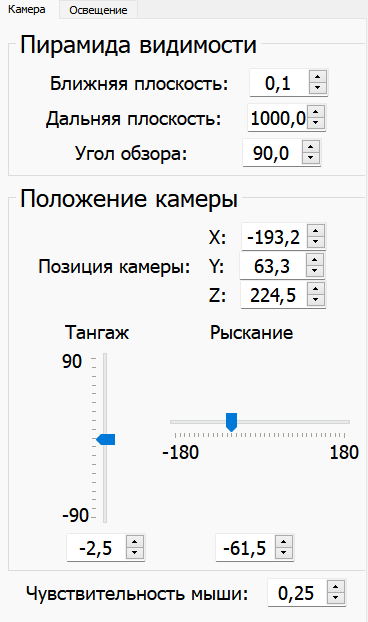
\includegraphics[width=0.27\textwidth]{img/examples/camera.png}
	\caption{Раздел камеры}
	\label{fig:camera}
\end{figure}

Раздел <<Освещение>> содержит положение и цвет источника освещения (рисунок~\ref{fig:light}). 
При выборе цвета появляется диалоговое окно с палитрой цветов (рисунок~\ref{fig:сhoose-color}).

\begin{figure}[h]
	\centering
	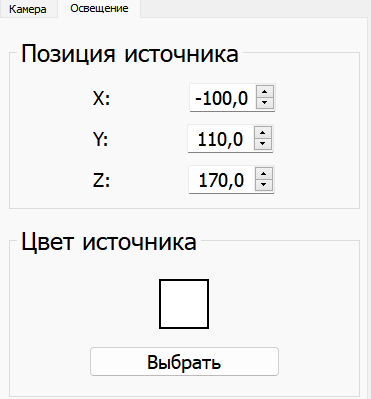
\includegraphics[width=0.5\textwidth]{img/examples/light.png}
	\caption{Раздел освещения}
	\label{fig:light}
\end{figure}

\begin{figure}[h]
	\centering
	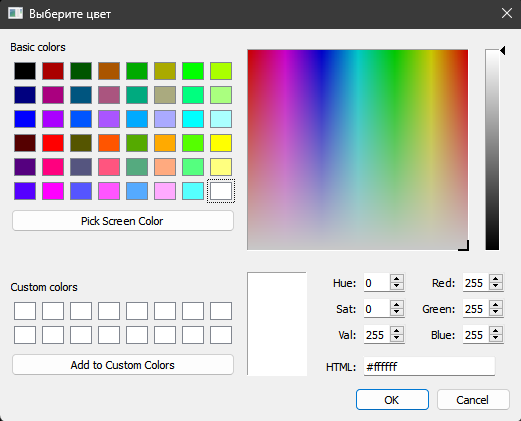
\includegraphics[width=0.5\textwidth]{img/examples/choose-color.png}
	\caption{Окно выбора цвета}
	\label{fig:сhoose-color}
\end{figure}

\clearpage

На рисунке~\ref{fig:example_work} приведен пример работы программы.

\begin{figure}[h]
	\centering
	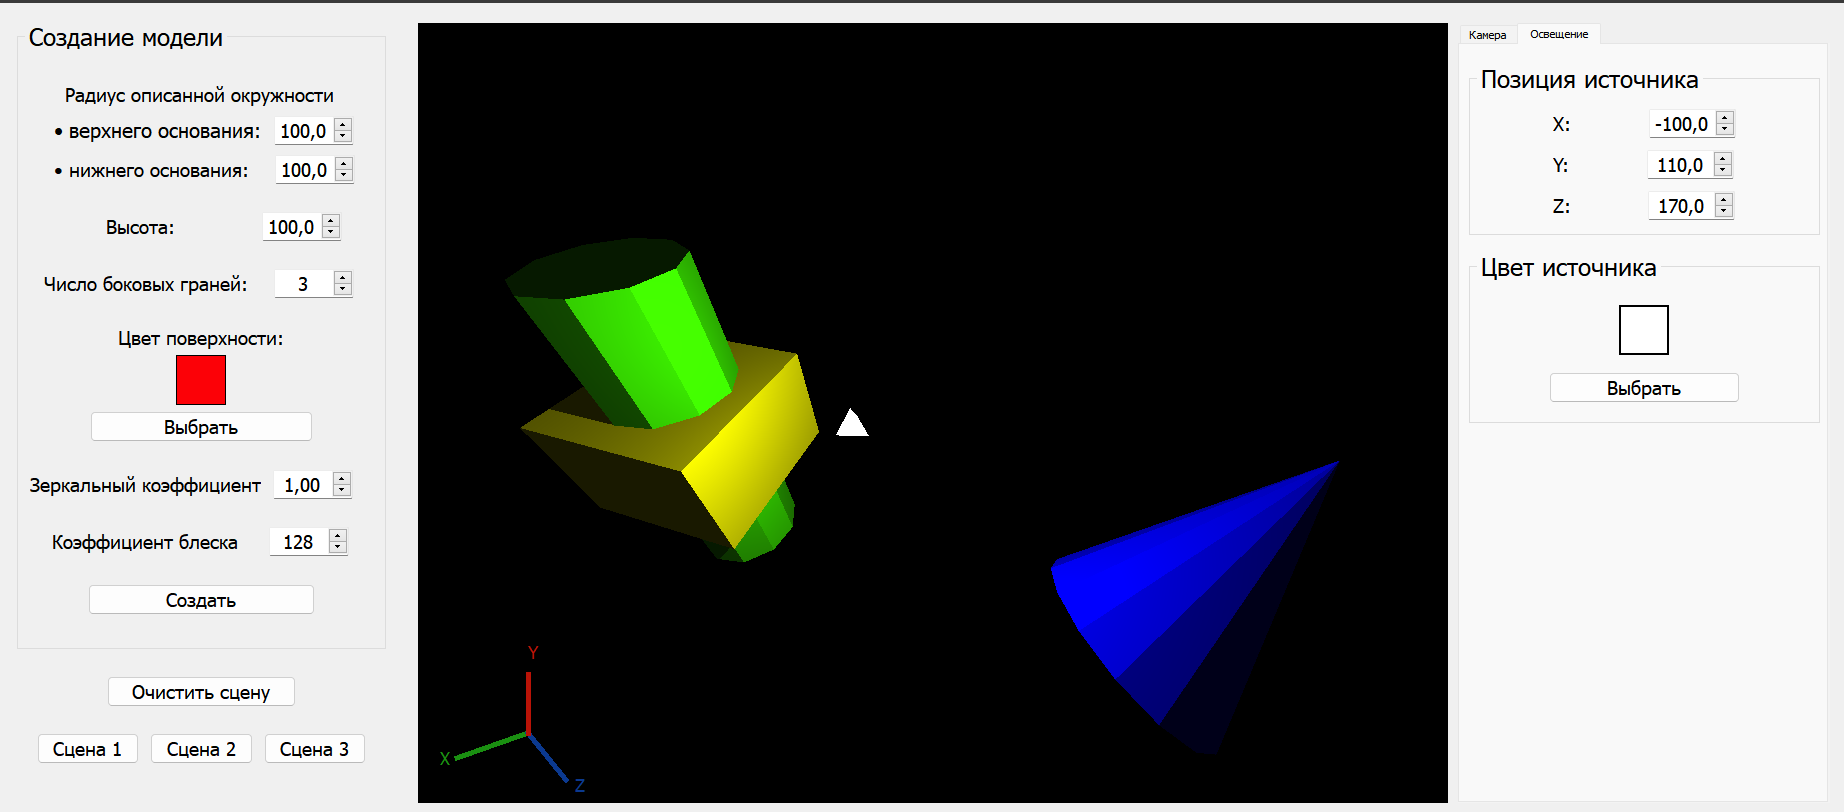
\includegraphics[width=0.95\textwidth]{img/examples/example-models.png}
	\caption{Тестовая сцена}
	\label{fig:example_work}
\end{figure}

\subsection*{Вывод}

В данном разделе были выбраны средства реализации, описаны структуры классов программы, описаны модули, а также рассмотрен интерфейс программы
